
\chapter{Lepton Efficiency Scale Factors}\label{ch:eff}
The efficiency of the trigger and reconstruction and identification steps for leptons is non-unity and differs between simulation and data. Determining the efficiency of the reconstruction and identification stages in simulation and data provides a scale factor $\epsilon_{data}/\epsilon_{MC}$ for each lepton to effectively match the reconstruction efficiency of simulation to data. The scale factor is applied to the simulated signal and background samples to emulate the lepton reconstruction and identification efficiency expected in data. Efficiency scale factors are derived for leptons in $|\eta|<2.4$ and $\pt>25\GeV$, with sufficient $\pt$ and $\eta$ granularity chosen to separate behavior in different kinematic regions and detector geometries. The factorization of the efficiency categories for electrons is shown in Equation~\ref{eq:ele_eff} and for muons in Equation~\ref{eq:mu_eff}.
\begin{equation}
  \epsilon_{e} = \epsilon_{GSF+Sel+ISO} \times \epsilon_{Trigger}
  \label{eq:ele_eff}
\end{equation}
\begin{equation}
  \epsilon_{\mu} = \epsilon_{Sel+ISO+Trk} \times  \epsilon_{Sta} \times \epsilon_{Trigger}
  \label{eq:mu_eff}
\end{equation}
The efficiency categories for electrons are:
\begin{itemize}
    \item $\epsilon_{GSF+Sel+ISO}$: Efficiency of reconstructing a GSF electron which passes the electron selection requirements
    \item $\epsilon_{Trigger}$: Efficiency of a GSF electron passing selection requirements being selected by the trigger
\end{itemize}
Likewise the categories for muons are:
\begin{itemize}
    \item $\epsilon_{Sta}$: Efficiency for a global muon to be matched to the standalone muon system
    \item $\epsilon_{Sel+Iso+Trk}$: Efficiency of a standalone muon to be matched to a global muon with tracker hits as well as satisfying the muon selection and isolation criteria
    \item $\epsilon_{Trigger}$: Efficiency of a fully reconstructed muon passing selection requirements also being selected by the trigger
\end{itemize}
In the simulated \zll events, it is further required that both of the leptons be matched with $\Delta R < 0.5$ to a generator-level lepton originating from the \Z boson. 


% %%%% Tables for Electron Efficiency SF Uncertainty for 13 TeV  %%%%%
\begin{table}%[htbp]
\begin{center}
\scalebox{0.7}{
\begin{tabular}{ccccc}
\hline
Probe Type & Tag Type & $\eta$ bins & $p_T$ bins & Charge bins \\
\hline \hline
GSF+Selection+Iso & sc  & 12 &  8 & charge-inclusive\\
Trigger & GSF electron  & 12 &  8  & +, -\\
\hline
\end{tabular}}
\end{center}
\caption{General implementation of the electron scale factor derivation. Both sets of scale factors are derived for $e^+$ and $e^-$ separately. }
\label{tab:Eff:Binning:Ele}
\end{table}

% %%%% Tables for Electron Efficiency SF Uncertainty for 13 TeV  %%%%%
\begin{table}%[htbp]
\begin{center}
\scalebox{0.7}{
\begin{tabular}{ccccc}
\hline
Probe Type & Tag Type & $\eta$ bins & $p_T$ bins & Charge bins\\
\hline \hline
Sel+ID+Iso & 0.00  & 12 &  3 &charge-inclusive\\
Standalone & 0.00  & 12 &  3  & charge-inclusive\\
Trigger & 0.00  & 12 &  8  & +, -\\
\hline
\end{tabular}}
\end{center}
\caption{General implementation of the muon scale factor derivation. Standalone efficiency has fewer $pT$ bins due to the low $p_T$ dependence and having a stastically limited fit in the failing probe category.}
\label{tab:Eff:Binning:Mu}
\end{table}



%% %%%%%%%%%%%%%%%%%%%%%%%%%%%
%%                Tag & Probe
%%%%%%%%%%%%%%%%%%%%%%%%%%%%%
\section{Tag and Probe}\label{ch:eff:tagandprobe}
A tag-and-probe method is employed on the \zll sample, with leptons required to have $\pt>25\GeV$ and $|\eta|<2.4$. \zll events provide a high-purity sample of high-\pt leptons which have similar kinematic properties to those also present in the leptonic \W boson decays\cite{Khachatryan:2010xn}. Tag leptons are required to pass the standard analysis selection cuts as well as be matched to the appropriate trigger. Probe leptons are then selected from leptons passing the loose kinematic cuts of $p_T > 25 \mathrm{~GeV}$,~$|\eta|<2.4$, and producing a tag+probe invariant mass in the range \masswindow. Probes are classified by their ability to pass a set of criteria depending on the efficiency category being studied. Calculation of the efficiency is described in Section~\ref{ch:eff:fitting}.

Lepton efficiencies are calculated based on the probe \pt and $\eta$. Binning by $\eta$ is listed in Table~\ref{tab:eff:bin:eta} and binning by $\pt$ is listed in Table~\ref{tab:eff:bin:pt}. Identical $(\pt,\eta)$ binning is used at \sg and \sh for a given category. The trigger efficiency for all channels is derived with positively and negatively charged categories separated, while the charges are combined for the other categories\cite{CMS:2020ksi}. Electron efficiency $\eta$ binning includes a category specifically to accommodate the gap between the endcap and barrel which contains a large amount of inactive material and has a significantly lower efficiency than other areas.
%%%% Tables for Electron Efficiency SF Uncertainty for 13 TeV  %%%%%
\begin{table}[htbp]
\begin{center}
\scalebox{0.9}{
\begin{tabular}{cc}
\hline
Channel~~ & $\eta$ bins \\
\hline \hline
Muon  & -2.4, -2.1, -1.6, -1.2, -0.9, -0.3, 0, 0.3, 0.9, 1.2, 1.6, 2.1, 2.4  \\
Electron  & -2.4, -2.0, -1.566, -1.4442, -1.0, -0.5, 0, 0.5, 1.0, 1.4442, 1.566, 2.0, 2.4 \\
\hline
\end{tabular}}
\end{center}
\caption{$\eta$ binning used for each lepton channel. }
\label{tab:eff:bin:eta}
\end{table}

%%%% Tables for Electron Efficiency SF Uncertainty for 13 TeV  %%%%%
\begin{table}[htbp]
\begin{center}
\scalebox{0.9}{
\begin{tabular}{ccc}
\hline
Category & ~Channel~ & \pt bins [\GeV] \\
\hline \hline
Trigger & electron, muon ~~`& 25, 26.5, 28, 29.5, 31, 32.5, 35, 40, 45, 50, 60, 80, $\infty$ \\
\hline
GSF+ID+Iso & electron  \\
Standalone & muon &  25, 35, 50, $\infty$ \\
Selection+Iso & muon &  \\
\hline
\end{tabular}}
\end{center}
\caption{\pt binning used for each efficiency category. }
\label{tab:eff:bin:pt}
\end{table}


% Category & ~~~$\ell$~~~ & \pt bins [\GeV] \\
% \hline \hline
% Trigger & $e, \mu$ & 25, 26.5, 28, 29.5, 31, 32.5, 35, 40, 45, 50, 60, 80, $\infty$ \\
% \hline
% GSF+ID+Iso & $e$ &  \\
% Standalone & $\mu$ &  25, 35, 50, $\infty$ \\
% Selection+Iso & $\mu$ &  \\



%% %%%%%%%%%%%%%%%%%%%%%%%%%%%
%%                Fitting
%%%%%%%%%%%%%%%%%%%%%%%%%%%%%

\section{Fitting Method}\label{ch:eff:fitting}
Probes are classified into a "pass" and "fail" category for efficiency type being studied. The number of passing and failing $Z\rightarrow ll$ events determine the efficiency as shown in Equation~\ref{eq:eff:eq}. For simulated samples, which are pure \zll, $N_{pass}$ and $N_{fail}$ can be determined by counting the number of events in each category per $(\pt,\eta)$ bin. 

\begin{equation}
\epsilon = \frac{N_{pass}}{N_{pass}+N_{fail}}
\label{eq:eff:eq}
\end{equation}
Data may also include background events in addition to the \zll signal events, particularly the failing probe categories which can have significant contributions from non-resonant backgrounds such as QCD. A fit is performed with the \zll signal described by the reconstructed \mll distribution from simulation convolved with a Gaussian, and a background described by an analytic function. The choice of analytic function depends on the category of efficiency, and more complicated functions are used to model effects in categories with larger background contributions. The primary background models are:
\begin{itemize}
\item \textbf{Exponential} (1 free parameter) for categories with relatively low background contribution. Used as background model for all 'pass' categories as well as the 'fail' category for muon selection+isolation+track efficiency.
\item \textbf{Gaussian Error function $\times$ Exponential} $f(x)=erf(b(a-x))e^{c(x-M_Z)}$\\ (3 free parameters) Used for 'fail' category of electron GSF+Selection efficiency. High \pt requirements for tag and probe result in kinematic turn-on in \mll spectrum, which can be described with this model.
\item \textbf{Quadratic polynomial} (3 free parameters) for muon standalone efficiency. This category has a lower resolution and relatively large background contribution in the failing probe category and cannot be fit with the exponential.
\end{itemize}
After construction of the signal and background models, the passing and failing categories for a given kinematic bin are simultaneously fit with Equations~\ref{eq:eff:pass:full} and~\ref{eq:eff:fail:full} to extract $\epsilon$. Examples of the fit are shown in Figure~\ref{fig:eff:musta:fitexample}.The events in the category of $\epsilon_{HLT}$ have negligible background, and $\epsilon$ is determined by counting events in the "pass" and "fail" categories.

\begin{equation}
F^{pass}\left(m_{ll}\right)=\epsilon \times N_{tot} \times F_{sig}^{pass}\left(m_{ll} \right) + N^{pass}_{bkg} \times F_{bkg}^{pass} \left(m_{ll} \right)
\label{eq:eff:pass:full}
\end{equation}
\begin{equation}
F^{fail}\left(m_{ll}\right)=\left(1-\epsilon\right) \times N_{tot} \times F_{sig}^{fail}\left(m_{ll} \right) + N^{fail}_{bkg} \times F_{bkg}^{fail} \left(m_{ll} \right)
\label{eq:eff:fail:full}
\end{equation}





%% %%%%%%%%%%%%%%%%%%%%%%%%%%%
%%                Systematics
%%%%%%%%%%%%%%%%%%%%%%%%%%%%%
\section{Modeling and Systematic Uncertainties}\label{ch:eff:systematics}
Uncertainties in the efficiency factors is evaluated for sources including signal model choice, background model choice, and tag selection. The variations in the scale factors is propagated to the discriminant distributions used in the final fit.
\subsection{Evaluating Model Differences}
Uncertainties in the scale factors are evaluated as coming from model-dependence of results on the signal and background shapes. These include the FSR model, generator, and background model. Additionally, the impact of the minimum tag selection \pt is evaluated. 
The impact of the model assumptions is evaluated by generating a set of simulated datasets from the \mll distribution describing the original efficiency model and fitting with the alternative models. The pull, $ (\epsilon_{meas}-\epsilon_{true})/{\sigma_{meas}} $, for each trial is calculated, and the mean pull per \pt-$\eta$ bin is taken to be the uncertainty due to the alternate model. 
% \begin{equation}
% \mathrm{pull}=\frac{\epsilon_{meas}-\epsilon_{true}}{\sigma_{meas}}
%     \label{eq:ch7:pull}
% \end{equation}

\subsubsection{Generator Model}

\textbf{\aMCATNLO vs. \POWHEG:} The primary signal simulation for this analysis is generated by  \MADGRAPH5\_\aMCATNLO interfaced to \PYTHIA8 for parton showering. One of the features of \aMCATNLO is that it allows for negative event weights arising from loop diagrams at NLO. Another event generator, \POWHEG, disallows this and instead calculates to LO in the kinematic region where negative values would appear. To estimate the kinematic differences between these two approaches, samples with \aMCATNLO and \POWHEG2 (both interfaced to \PYTHIA8 for parton showering) are compared. New signal models are created from the \POWHEG \mll distributions convolved with a Gaussian.

\subsubsection{Final-State Radiation Model}
\textbf{\PYTHIA vs. \PHOTOS:} Final state radiation and higher-order electroweak corrections for the main set of simulations is performed by \PYTHIA8. As described in Chapter~\ref{ch:ewkcorr}, differences in the order of FSR and electroweak corrections are estimated by comparing \PYTHIA and \PHOTOS with both interfaced to \POWHEG. Post-FSR information from these samples are used to reweight the reconstructed  \mll distributions from the primary \aMCATNLO+\PYTHIA8 simulation. The reweighted \mll distributions are used to create alternative fitting models.

\subsubsection{Background Model}\label{ch:eff:bkg}
The \zll events generally provide a clean signature with minimal background, but there can be significant backgrounds from QCD or W+jets primarily appearing in the probes failing the reconstruction and selection categories. In the fits, the backgrounds are modeled with analytic functions as described below. 
\begin{itemize}
\item \textbf{exponential} for all passing categories and muon selection+isolation+track efficiency
\item \textbf{exponential $\times$ erf} for electron GSF ID+Isolation efficiency 
\item \textbf{quadratic polynomial} for muon standalone efficiency failing probes
\end{itemize}
The alternate set of fitting functions is constructed with:
\begin{itemize}
\item \textbf{power law} $f(x)\propto x^{-k},k\geq0$ for alternative model in all categories. Able to describe the falling \mll spectrum in the low-background categories as well as the 
\end{itemize}
Examples of a muon standalone efficiency fit using the standard quadratic function and the alternative power law model are shown in Figure~\ref{fig:eff:musta:fitexample}. 

%%%% Figures for ZeeGSFSel Efficiency  %%%%%
\begin{figure}
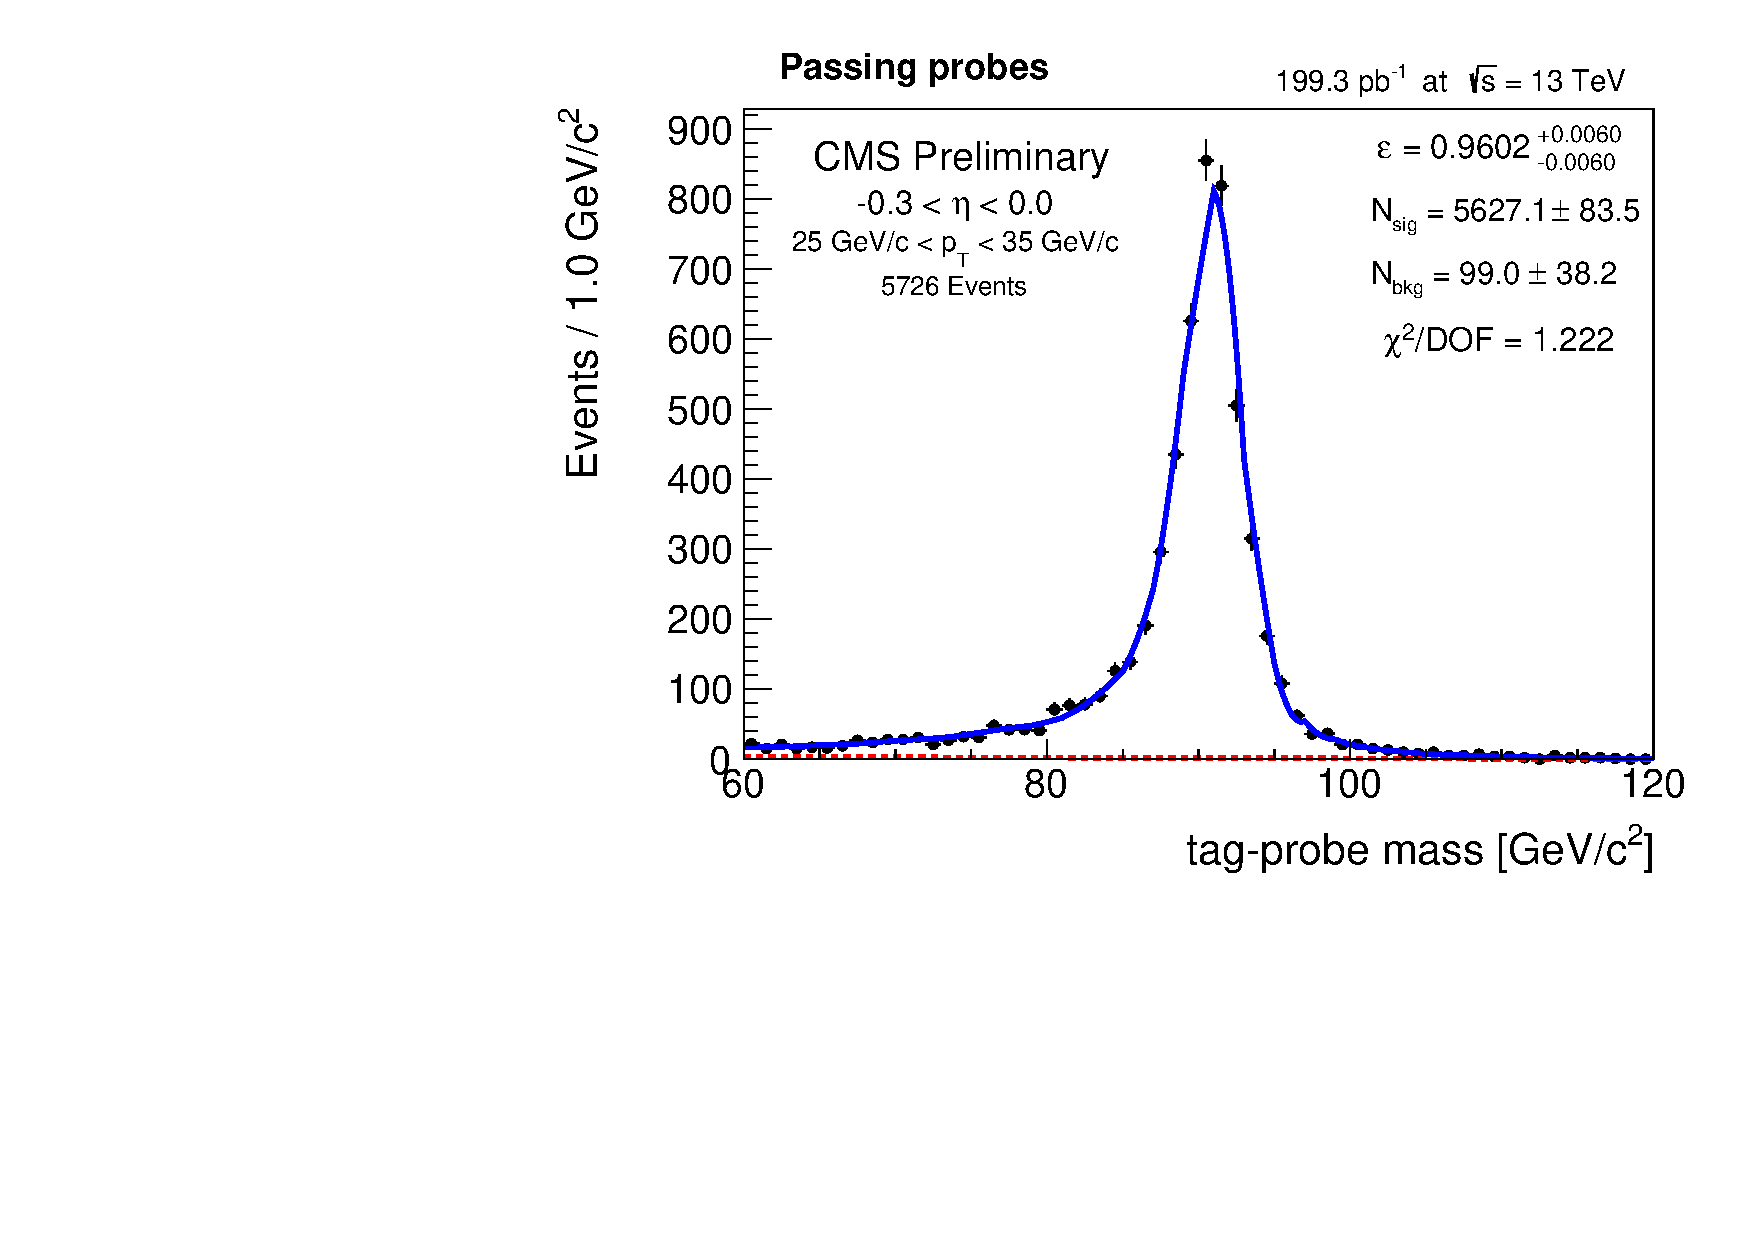
\includegraphics[width=.49\linewidth]{plots/efficiency/examples_musta/passetapt_5.pdf}
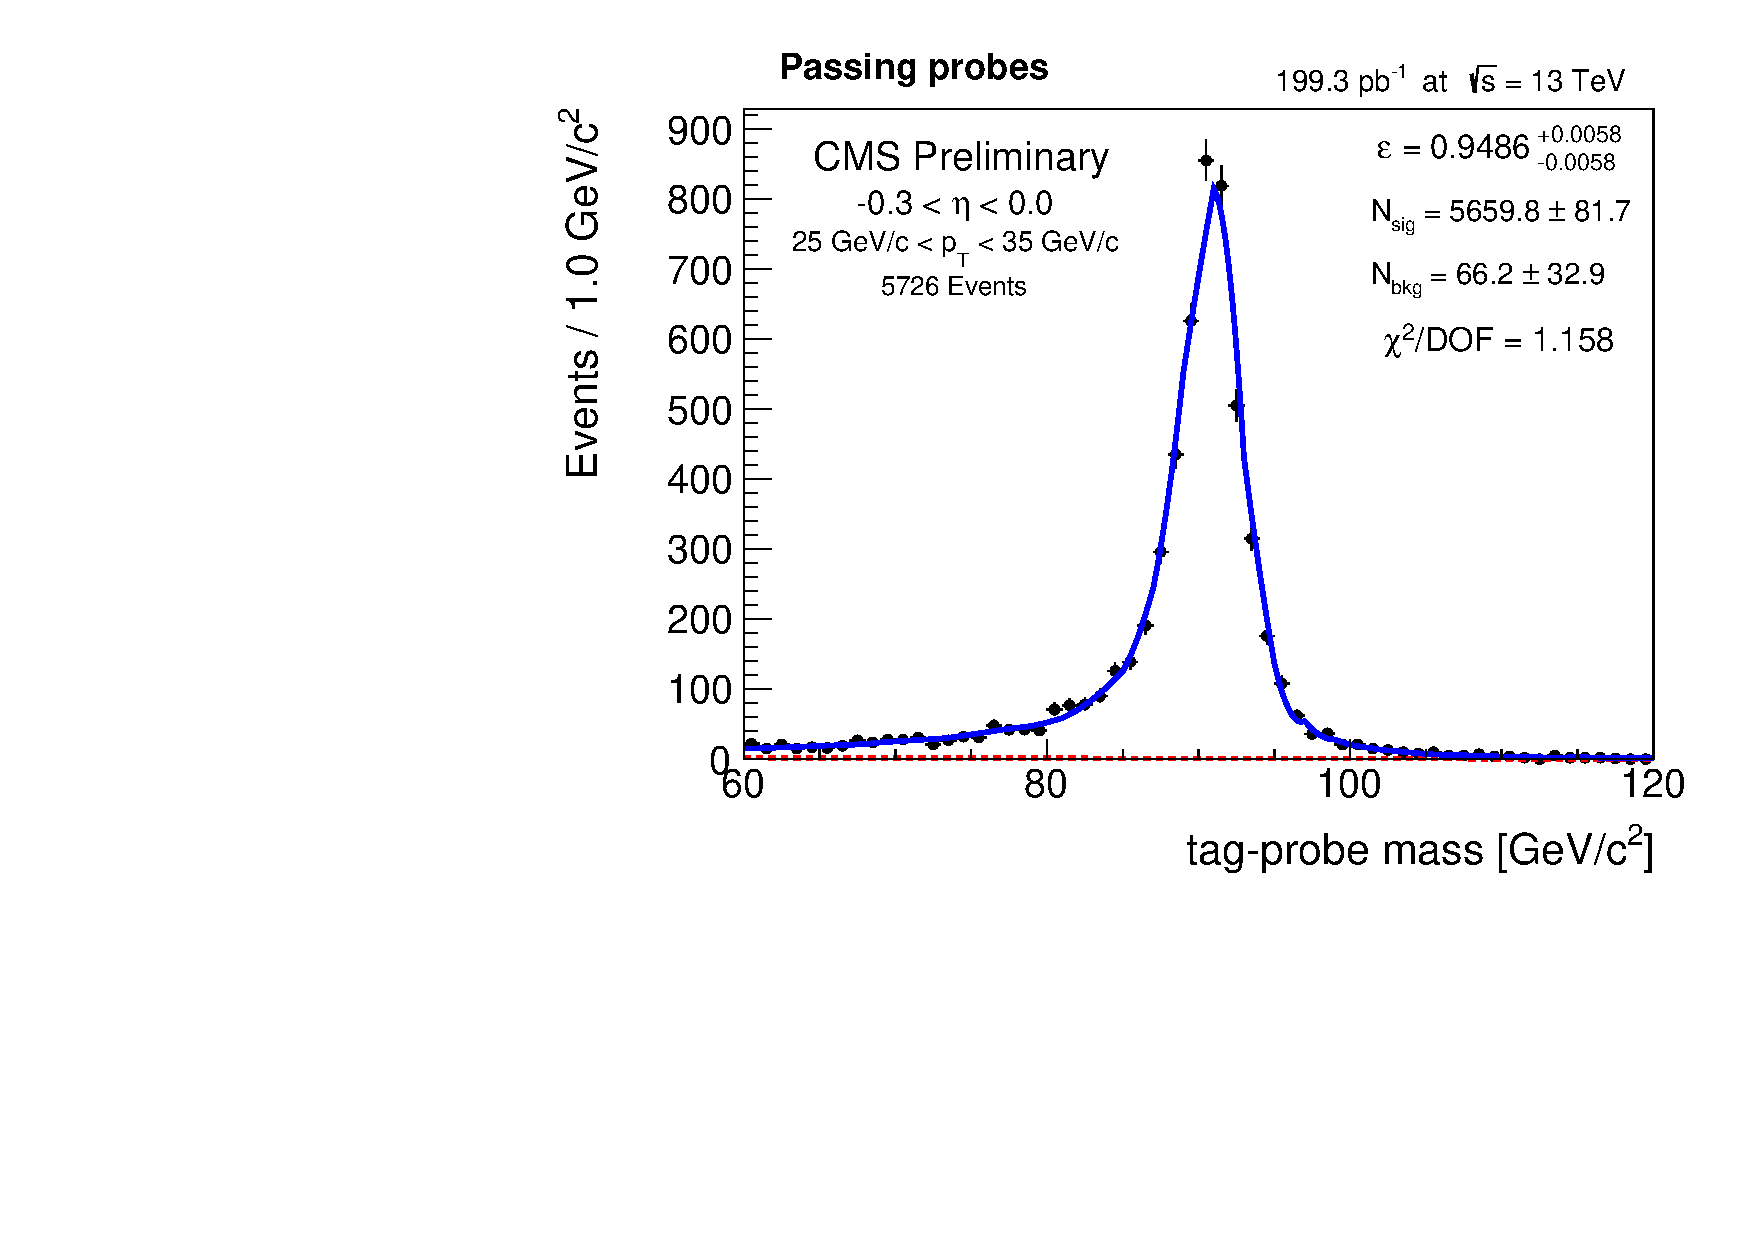
\includegraphics[width=.49\linewidth]{plots/efficiency/examples_plbkg/passetapt_5.pdf}
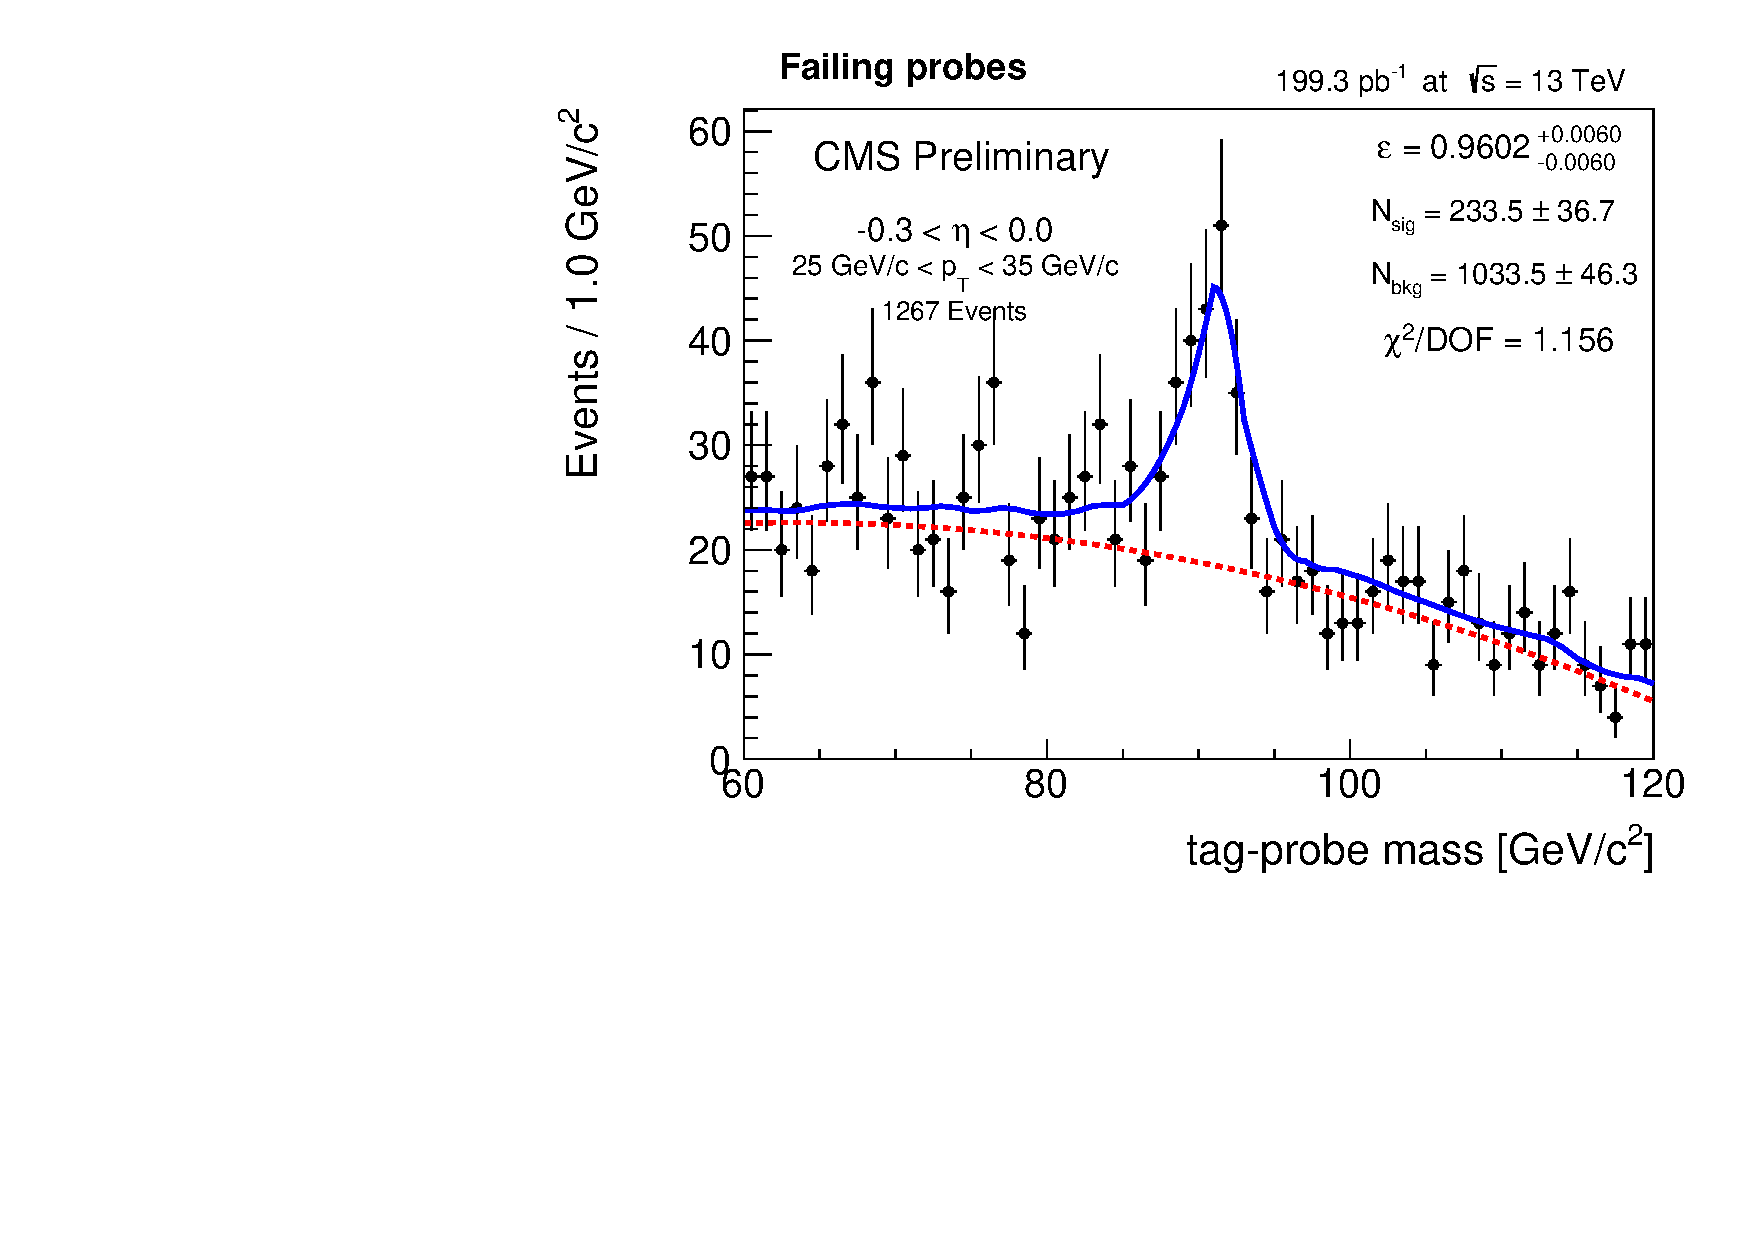
\includegraphics[width=.49\linewidth]{plots/efficiency/examples_musta/failetapt_5.pdf}
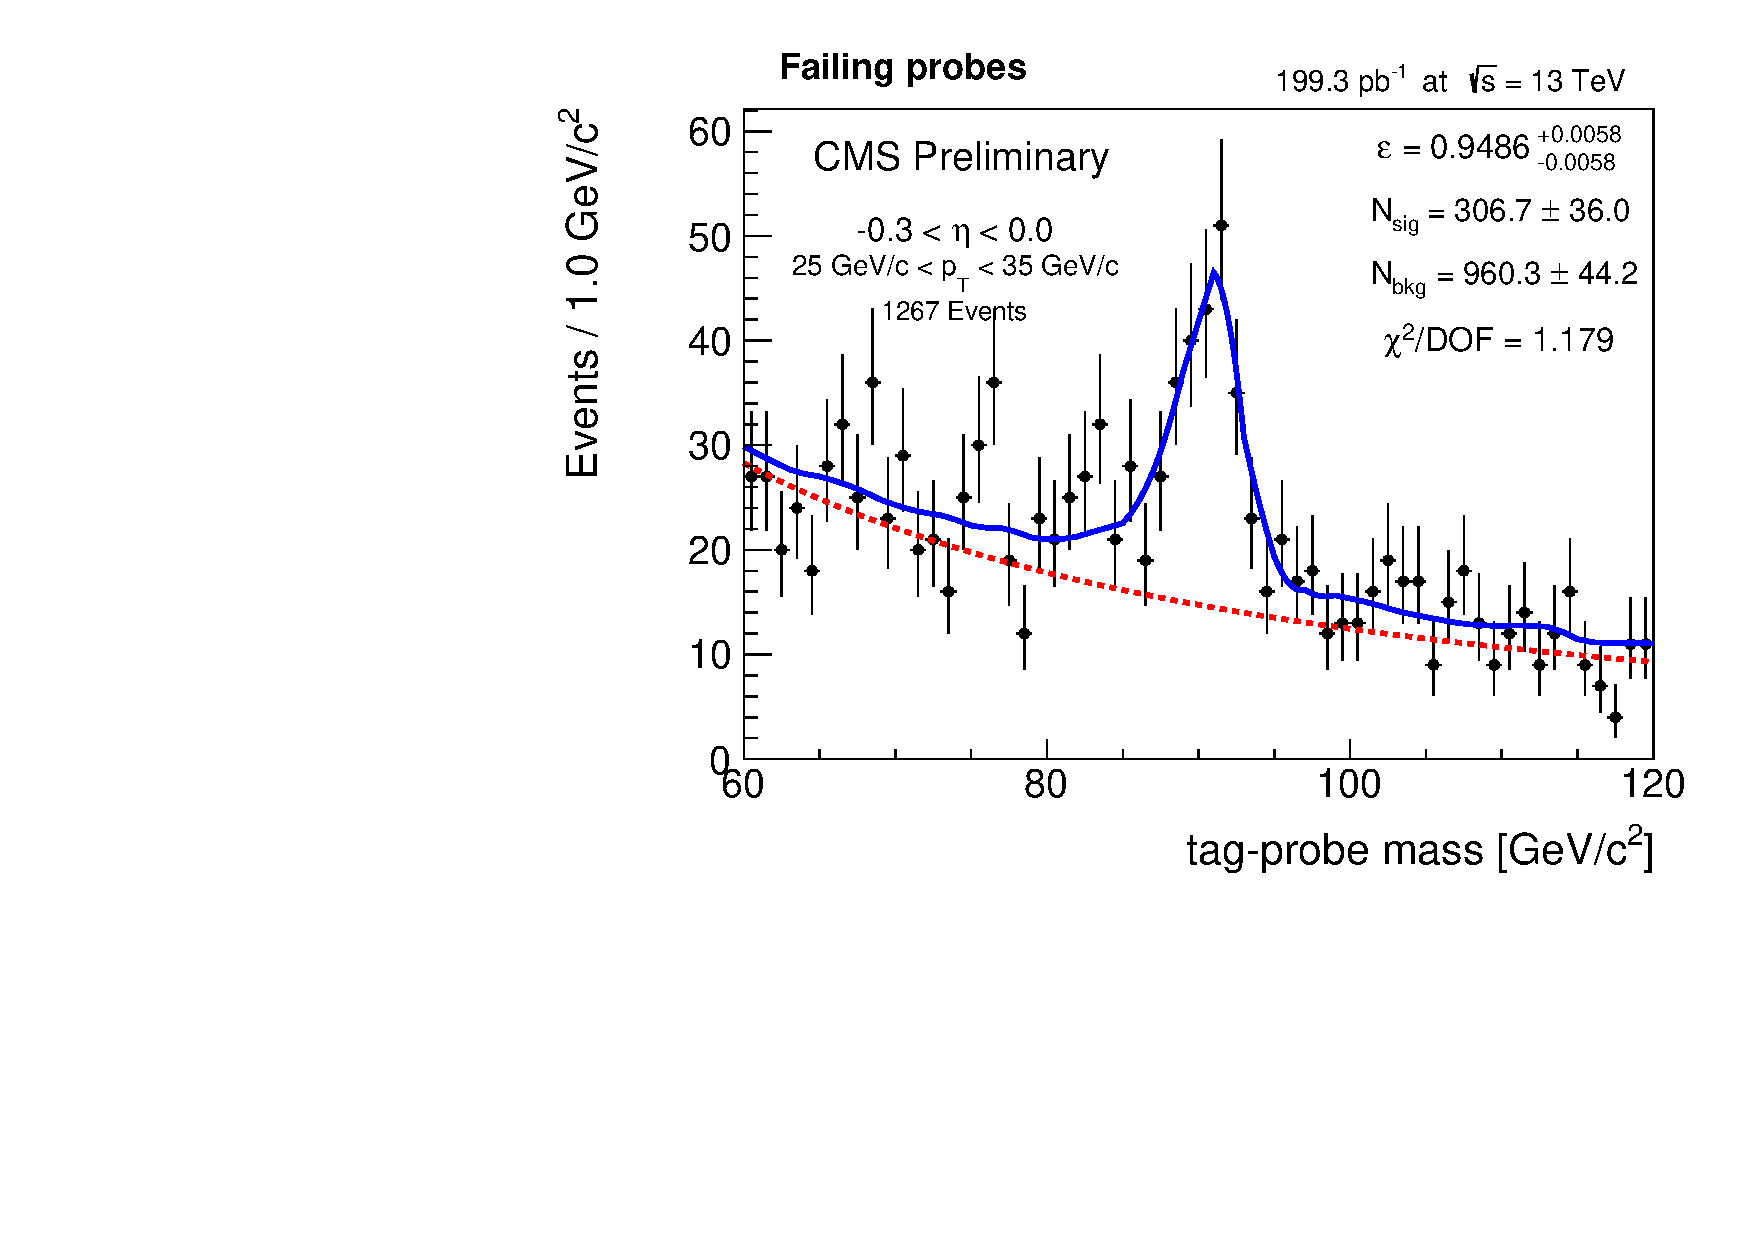
\includegraphics[width=.49\linewidth]{plots/efficiency/examples_plbkg/failetapt_5.pdf}
\caption{Examples of passing (top) and failing (bottom) probes from the same $p_T-\eta$ bin, from the muon standalone efficiency, fit with two different background models. The left plots use a quadratic polynomial and the right plots use a power law (shown in red).}
\label{fig:eff:musta:fitexample}
\end{figure}


\subsubsection{Tag Selection Uncertainty}
Uncertainty due to the selection criteria of the tag lepton are evaluated by directly comparing the impact of efficiency scale factors using the standard cut ($\pt > 25 \GeV$) to efficiency scale factors derived using tag leptons with $\pt > 30\GeV$. 

% \subsection{Summary of Systematic Uncertainties}
% A summary of the systematic uncertainties on the efficiency scale factors can be found in the Systematics Chapter later. 
% The impact of alternate models is evaluated by propagating the difference between models as a modification to the efficiency scale factor, and computing the selection-level acceptance with each of the alternative efficiency models. 
% Contributions of each type of systematic uncertainty are listed in the Tables ~\ref{tab:Eff:Unc:muon:summary:13} and ~\ref{tab:Eff:Unc:ele:summary:13} for 13 TeV and Table~\ref{tab:Eff:Unc:ele:summary:5} and Table~\ref{tab:Eff:Unc:mu:summary:5} for 5 TeV. 

\subsection{Statistical Uncertainty}
Statistical uncertainties in the efficiency scale factor are taken from the average over all variations on the measurement. The statistical uncertainty for a single $(\pt,\eta)$ bin is treated as Poisson, as given in Ref.~\cite{Paterno:2004cb}. Uncertainties for a given $(\pt,\eta)$ bin are correlated across all events containing leptons in the bin, while the uncertainties from separate $(\pt,\eta)$ bins are treated as uncorrelated. Individual categories (reconstruction, identification and isolation, trigger, etc.) are also treated as uncorrelated. The overall impact on the signal yield from the efficiency scale factor statistical uncertainties for the electron and muon channels in \sg and \sh are listed in Table~\ref{tab:eff:stat:all}.
%%%% Table containing the $e$ ID+Iso cuts
\begin{table}%[htbp]
\begin{center}

\scalebox{1.0}{
\begin{tabular}{|c|c|c|}
\hline
(13 TeV) & electron [\%] & muon [\%]\\
\hline \hline
$W^+$     & 0.489 & 0.291 \\
$W^-$     & 0.485 & 0.278 \\
$Z$       & 0.498 & 0.283 \\
\hline
\end{tabular} }
\quad
\scalebox{1.0}{
\begin{tabular}{|c|c|c|}
\hline
(5 TeV) & electron [\%] & muon [\%]\\
\hline \hline
$W^+$     & 0.489 & 0.245 \\
$W^-$     & 0.471 & 0.231\\
$Z$       & 0.526 & 0.268 \\
\hline
\end{tabular} }

\end{center}

\caption{Statistical uncertainty [\%] in the efficiency scale factor calculations on the \Wp, \Wm, and \Z boson acceptance at \sh (left) and \sg (right).}
\label{tab:eff:stat:all}
\end{table}

\begin{table}[htbp]
\begin{center}
\begin{tabular}{ccccccccc}
\hline
Source & $W^+$& $W^-$ & $W$ & $W^+/W^-$ & $Z$ & $W^+/Z$&$W^+/Z$ &$W/Z$  \\
\hline \hline
FSR & 0.191 & 0.169 & 0.181 & 0.021 & 0.238 & 0.049 & 0.070 & 0.058 \\
MC & 0.073 & 0.067 & 0.070 & 0.006 & 0.094 & 0.023 & 0.029 & 0.025 \\
Background & 0.007 & 0.008 & 0.008 & 0.000 & 0.012 & 0.002 & 0.002 & 0.002 \\
Tag pT & 0.033 & 0.038 & 0.035 & 0.004 & 0.093 & 0.058 & 0.054 & 0.056 \\
Statistical & 0.286 & 0.278 & 0.202 & 0.009 & 0.279 & 0.008 & 0.001 & 0.076 \\
\hline \hline
Total [\%] & 0.35 & 0.33 & 0.28 & 0.00 & 0.39 & 0.07 & 0.08 & 0.10 \\

\end{tabular}
\end{center}
\caption{Uncertainties on the lepton efficiency scale factors for the muon channel in 13 TeV}
\label{tab:Eff:Unc:muon:summary:13}
\end{table}

\begin{table}[htbp]
\begin{center}
\begin{tabular}{ccccccccc}
\hline
Source & $W^+$& $W^-$ & $W$ & $W^+/W^-$ & $Z$ & $W^+/Z$&$W^+/Z$ &$W/Z$  \\
\hline \hline
FSR & 0.081 & 0.080 & 0.081 & 0.001 & 0.166 & 0.087 & 0.089 & 0.085 \\
MC & 0.057 & 0.057 & 0.056 & 0.000 & 0.093 & 0.038 & 0.038 & 0.036 \\
Background & 0.056 & 0.053 & 0.055 & 0.004 & 0.099 & 0.041 & 0.044 & 0.045 \\
Tag pT & 0.016 & 0.018 & 0.017 & 0.001 & 0.047 & 0.066 & 0.067 & 0.063 \\
Statistical & 0.489 & 0.486 & 0.349 & 0.001 & 0.488 & 0.002 & 0.003 & 0.137 \\
\hline \hline
Total [\%] & 0.50 & 0.50 & 0.36 & 0.00 & 0.53 & 0.11 & 0.11 & 0.18 \\


\end{tabular}
\end{center}
\caption{Uncertainties on the lepton efficiency scale factors for the electron channel in 13 TeV}
\label{tab:Eff:Unc:ele:summary:13}
\end{table}
%%%% Summary of lep eff systematics for muons - 5 TeV  %%%%%
\begin{table}[htbp]
\begin{center}
\begin{tabular}{ccccccccc}
\hline
Source & $W^+$& $W^-$ & $W$ & $W^+/W^-$ & $Z$ & $W^+/Z$&$W^+/Z$ &$W/Z$  \\
\hline \hline
MC & 0.09 & 0.08 & 0.09 & 0.00 & 0.15 & 0.07 & 0.07 & 0.07 \\
FSR & 0.17 & 0.15 & 0.32 & 0.01 & 0.27 & 0.23 & 0.26 & 0.24 \\
Bkg Model & 0.01 & 0.01 & 0.01 & 0.01 & 0.00 & 0.01 & 0.01 & 0.01 \\
Tag pT & 0.48 & 0.49 & 0.48 & 0.01 & 0.88 & 0.45 & 0.45 & 0.45 \\
stat & 0.25 & 0.24 & 0.20 & 0.32 & 0.26 & 0.38 & 0.36 & 0.35 \\
 \\
\hline \hline
Total [\%] & 0.56 & 0.56 & 0.61 & 0.32 & 0.96 & 0.62 & 0.62 & 0.61 \\
\end{tabular}
\end{center}
\caption{Summary of the propagated muon efficiency systematic uncertainties at 5 TeV.}
\label{tab:Eff:Unc:mu:summary:5}
\end{table}

%%%% Summary of lep eff systematics for electrons - 5 TeV  %%%%%
\begin{table}%[htbp]
\begin{center}
\scalebox{0.7}{
\begin{tabular}{ccccccccc}
\hline
Source & $W^+$& $W^-$ & $W$ & $W^+/W^-$ & $Z$ & $W^+/Z$&$W^+/Z$ &$W/Z$  \\
\hline \hline
Binning [\%] & 0.00  & 0.00 & 0.00 & 0.00 & 0.00& 0.00& 0.00& 0.00\\
Signal Shape [\%] & 0.00  & 0.00 & 0.00 & 0.00 & 0.00& 0.00& 0.00& 0.00 \\
Background Shape [\%] & 0.00  & 0.00 & 0.00 & 0.00 & 0.00& 0.00& 0.00& 0.00  \\
\hline
\end{tabular}}
\end{center}
\caption{Summary of the propagated electron efficiency systematic uncertainties at 5 TeV.}
\label{tab:Eff:Unc:ele:summary:5}
\end{table}

% %%%% Summary of lep eff systematics for electrons - 13/5 TeV ratios  %%%%%
\begin{table}%[htbp]
\begin{center}
\scalebox{0.7}{
\begin{tabular}{ccccccccc}
\hline
Source & $W^+$& $W^-$ & $W$ & $W^+/W^-$ & $Z$ & $W^+/Z$&$W^+/Z$ &$W/Z$ \\
\hline \hline
Binning [\%] & 0.00  & 0.00 & 0.00 & 0.00 & 0.00& 0.00& 0.00& 0.00 \\
Signal Shape [\%] & 0.00  & 0.00 & 0.00 & 0.00 & 0.00& 0.00& 0.00& 0.00 \\
Background Shape [\%] & 0.00  & 0.00 & 0.00 & 0.00 & 0.00& 0.00& 0.00& 0.00  \\
\hline
\end{tabular}}
\end{center}
\caption{Summary of the propagated electron efficiency systematic uncertainties for the 13TeV/5TeV ratio.}
\label{tab:Eff:Unc:ele:summary:13to5}
\end{table}

% %%%% Summary of lep eff systematics for muons - 13/5 TeV ratios  %%%%%
\begin{table}%[htbp]
\begin{center}
\scalebox{0.7}{
\begin{tabular}{ccccccccc}
\hline
Source & $W^+$& $W^-$ & $W$ & $W^+/W^-$ & $Z$ & $W^+/Z$&$W^+/Z$ &$W/Z$  \\
\hline \hline
Binning [\%]          & 0.00  & 0.00 & 0.00 & 0.00 & 0.00& 0.00& 0.00 & 0.00 \\
Signal Shape [\%]     & 0.00  & 0.00 & 0.00 & 0.00 & 0.00& 0.00& 0.00 & 0.00 \\
Background Shape [\%] & 0.00  & 0.00 & 0.00 & 0.00 & 0.00& 0.00& 0.00 & 0.00  \\
\hline
\end{tabular}
}
\end{center}
\caption{Summary of the propagated muon efficiency systematic uncertainties for the 13 Tev/5 TeV ratio.}
\label{tab:Eff:Unc:mu:summary:13to5}
\end{table}




%% %%%%%%%%%%%%%%%%%%%%%%%%%%%
%%                Results
%%%%%%%%%%%%%%%%%%%%%%%%%%%%%
\section{Results}\label{ch:eff:results}
% Overall efficiency scale factor effects for each of the \Wp, \Wm, and \Z boson channels at \sg and \sh is listed in Table~\ref{tab:Eff:Impact}. 
Tables listing the scale factors for each category and $(\pt,\eta)$ bin and figures comparing the efficiencies in data and simulation are provided in Appendix~\ref{ch:app:eff}.
